\section{Boolean Set-Operations on General Polygons\label{bso_sec:bso_gen}}
% ==================================================

\lcTex{%
  \setlength{\BooleanSetOpsWidthRight}{1.4cm}
  \setlength{\BooleanSetOpsWidthLeft}{\BooleanSetOpsWidthLineReal}
  \addtolength{\BooleanSetOpsWidthLeft}{-\BooleanSetOpsWidthRight}
  \begin{minipage}{\BooleanSetOpsWidthLeft}
}
\label{fig:general_polygon}
\begin{ccHtmlOnly}
  <p><center>
    <img src="./fig/general_polygon.gif" border=0 alt="A general polygon" align=right>
  </center>
\end{ccHtmlOnly}
In previous sections only ordinary (linear) polygons were dealt with. Namely, closed
point sets bounded by piecewise linear curves. The Boolean
set-operations package allows a more general geometric mapping of the
polygon edges. The operations provided by the package operate on point
sets bounded by $x$-monotone segments of general curves (e.g., conic
arcs and segments of polynomial functions). For example, the point set
depicted on the right is a general polygon bounded by two $x$-monotone
circular arcs that correspond to the lower half and the upper half of
a circle, respectively.
\lcTex{%
  \end{minipage}\hspace{\BooleanSetOpsMinipageSpace}
  \begin{minipage}{\BooleanSetOpsWidthRight}
    \begin{center}
    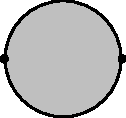
\includegraphics{Boolean_set_operations_2/fig/general_polygon}
    \end{center}
%    A general polygon.
  \end{minipage}
  \vspace{2pt}
}

Using the topological terminology, a general polygon can represent any
simply-connected point set whose boundary is a strictly simple curve.
Such a polygon is a model of the \ccc{GeneralPolygon_2} concept. A model
of this concept must fulfill the following requirements:
\begin{itemize}
\item A general polygon is constructible from a range of pairwise
interior disjoint $x$-monotone curves $c_1, \ldots, c_n$. The target
point of the $k$th curve $c_k$ and the source point of the next curve
in the range (in a cyclic order) must coincide, such that this point
defines the $k$th polygon vertex. 
\item It is possible to traverse the $x$-monotone curves that form the
edges of a general polygon.
\end{itemize}

\lcTex{%
  \setlength{\BooleanSetOpsWidthRight}{1.4cm}
  \setlength{\BooleanSetOpsWidthLeft}{\BooleanSetOpsWidthLineReal}
  \addtolength{\BooleanSetOpsWidthLeft}{-\BooleanSetOpsWidthRight}
  \begin{minipage}{\BooleanSetOpsWidthLeft}
}
\label{fig:general_polygon_with_holes}
\begin{ccHtmlOnly}
  <p><center>
    <img src="./fig/general_polygon_with_holes.gif" border=0 alt="A general polygon with holes" align=right>
  </center>
\end{ccHtmlOnly}
The concept \ccc{GeneralPolygonWithHoles_2} is defined in an analogous
way to the definition of linear polygons with holes. A model of this
concept represent a bounded or an unbounded set that may not be simply
connected, and must provide the following operations:
\lcTex{%
  \end{minipage}\hspace{\BooleanSetOpsMinipageSpace}
  \begin{minipage}{\BooleanSetOpsWidthRight}
    \begin{center}
    
\includegraphics{Boolean_set_operations_2/fig/general_polygon_with_holes}
    \end{center}
%    A general polygon with holes.
  \end{minipage}
  \vspace{1pt}
}
\begin{itemize}
\item Construction for a general polygon that represent the outer boundary
and a range of general polygons that represent the holes.
\item Accessing the general polygons that represents the outer boundary
(in case of a bounded set).
\item Traversing the holes.
\end{itemize}
In Section~\ref{bso_sec:bso_lin} we introduce the classes
\ccc{Polygon_2} and \ccc{Polygon_with_holes_2} that model the concepts
\ccc{GeneralPolygon_2} and \ccc{GeneralPolygonWithHoles_2}
respectively. In this section we introduce other models of these two
concepts.

The central class-template \ccc{General_polygon_set_2<Traits,Dcel>} is 
used to represent point sets that are comprised of a finite number of 
pairwise disjoint general polygons with holes, and provides various 
Boolean set-operations on such sets. It is parameterized by a {\em traits}
class and a \dcel{} class. The former defines the type of points used 
to represent polygon vertices and the type of $x$-monotone curves that 
represent the polygon edges. The traits class also provides primitive 
geometric operations that operate on objects of these types. 
The \dcel{} class is used to represent the underlying internal 
\ccc{Arrangement_2} data structure. The instantiated \ccc{Dcel} type is 
used to represent the underlying internal arrangement. It must model the 
concept \ccc{GeneralPolygonSetDcel}, and defaults to \ccc{Gps_default_dcel}.
You can override this default, with a different {\sc Dcel} class, typically
an extension of the default. Overriding the default is necessary only if 
you intend to obtain the underlying internal arrangement and process it further.

An instantiated
\ccc{General_polygon_set_2} class defines the nested types 
\ccc{General_polygon_set_2<Traits,Dcel>::Polygon_2} and
\ccc{General_polygon_set_2<Traits,Dcel>::Polygon_with_holes_2}, which model
the concepts \ccc{GeneralPolygon_2} and
\ccc{GeneralPolygonWithHoles_2} respectively.

% ------------------------------------
\subsection{The Traits-Class Concepts\label{bso_ssec:traits_concepts}}
% ------------------------------------

The traits class used to instantiate the \ccc{General_polygon_set_2}
class template must model the concept \ccc{GeneralPolygonSetTraits_2},
and is tailored to handle a specific family of curves. The concept
\ccc{GeneralPolygonSetTraits_2} refines the concept
\ccc{ArrangementDirectionalXMonotoneTraits_2} specified next.

The concept \ccc{ArrangementDirectionalXMonotoneTraits_2} refines the 
concept \ccc{ArrangementXMonotoneTraits_2} (see 
Section~\ref{arr_sssec:insert_x_mon} in the 2D Arrangements chapter).
Thus, a model of this concept must define the type \ccc{X_monotone_curve_2}, 
which represents an $x$-monotone curve, and the type \ccc{Point_2}, 
with represents a planar point. Such a point may be an endpoint of an
$x$-monotone curve or an intersection point between two curves.
It must also provide various geometric predicates and operations 
on these types listed by the base concept, such as determining whether
a point lies above or below an $x$-monotone curve, computing the
intersections between two curves, etc. Note that the base concept does
not assume that $x$-monotone curves are directed: an $x$-monotone
curve is not required to have a designated {\em source} and {\em
target}, it is only required to determine the left (lexicographically
smaller) and the right (lexicographically larger) endpoints of a given
curve.

The \ccc{ArrangementDirectionalXMonotoneTraits_2} concept treats its
$x$-monotone curves as directed objects. It thus requires two additional
operations on $x$-monotone curves:
\begin{itemize}
\item Given an $x$-monotone curve, compare its source and target points
lexicographically.
\item Given an $x$-monotone curve, construct its opposite curve (namely,
swap its source and target points).
\end{itemize}

The traits classes \ccc{Arr_segment_traits_2}, 
\ccc{Arr_non_caching_segment_traits}, \ccc{Arr_circle_segment_traits_2},
\ccc{Arr_conic_traits_2} and \ccc{Arr_rational_arc_traits_2}, which are 
bundled in the \ccc{Arrangement_2} package and distributed with \cgal,
are all models of the refined concept 
\ccc{ArrangementDirectionalXMonotoneTraits_2}.\footnote{The
\ccc{Arr_polyline_traits_2} class is {\em not} a model of the, 
\ccc{ArrangementDirectionalXMonotoneTraits_2} concept, as the
$x$-monotone curve it defines is always directed from left to
right. Thus, an opposite curve cannot be constructed. However, it is
not very useful to construct a polygon whose edges are polylines, as
an ordinary polygon with linear edges can represent the same entity.}

Just as with the case of computations using models of the 
\ccc{ArrangementXMonotoneTraits_2} concept, operations are robust only
when exact arithmetic is used. When inexact arithmetic is used,
(nearly) degenerate configurations may result in abnormal termination
of the program or even incorrect results.

% ---------------------------------------------------
\subsection{Operating on Polygons with Circular Arcs\label{bso_ssec:circ_seg}}
% ---------------------------------------------------

Two traits classes are distributed with \cgal. The first one is named
\ccc{Gps_segment_traits_2}, and it is used to perform Boolean
set-operations on ordinary polygons and polygons with holes. In fact,
the class \ccc{Polygon_set_2} introduced in
Section~\ref{bso_ssec:main_component} is a specialization of
\ccc{General_polygon_set_2<Gps_segment_traits_2>}. This class defined
its polygon and polygon with holes types, such that the usage of this
traits class is encapsulated in the polygon-set class.

The other predefined traits class is named 
\ccc{Gps_circle_segment_traits_2<Kernel>} and is parameterized by a
geometric \cgal\ kernel. By instantiating the \ccc{General_polygon_set_2}
with this traits class, we obtain the representation of a polygon whose
boundary may be comprised of line segments and circular arcs.
The circle--segment traits class provides predicates and constructions
on non-linear objects; yet, it uses only rational arithmetic and is
very efficient as a consequence.

\lcTex{%
  \setlength{\BooleanSetOpsWidthRight}{2.4cm}
  \setlength{\BooleanSetOpsWidthLeft}{\BooleanSetOpsWidthLineReal}
  \addtolength{\BooleanSetOpsWidthLeft}{-\BooleanSetOpsWidthRight}
  \begin{minipage}{\BooleanSetOpsWidthLeft}
}
\label{fig:circle_recs}
\begin{ccHtmlOnly}
  <p><center>
    <img src="./fig/circles_rects.gif" border=0 alt="Union of circles
    and rectangles" align=right>
  </center>
\end{ccHtmlOnly}
The following example uses the \ccc{Gps_circle_segment_traits_2} class
to compute the union of four rectangles and four circles. Each circle
is represented as a general polygon having two $x$-monotone circular arcs.
The union is computed incrementally, resulting with a single polygon with
a single hole, as depicted on the right. Note that as the four circles
are disjoint, their union is computed with the \ccc{insert} method,
while the union with the rectangles is computed with the \ccc{join}
operator.
\lcTex{%
  \end{minipage}\hspace{\BooleanSetOpsMinipageSpace}
  \begin{minipage}{\BooleanSetOpsWidthRight}
    \begin{center}
    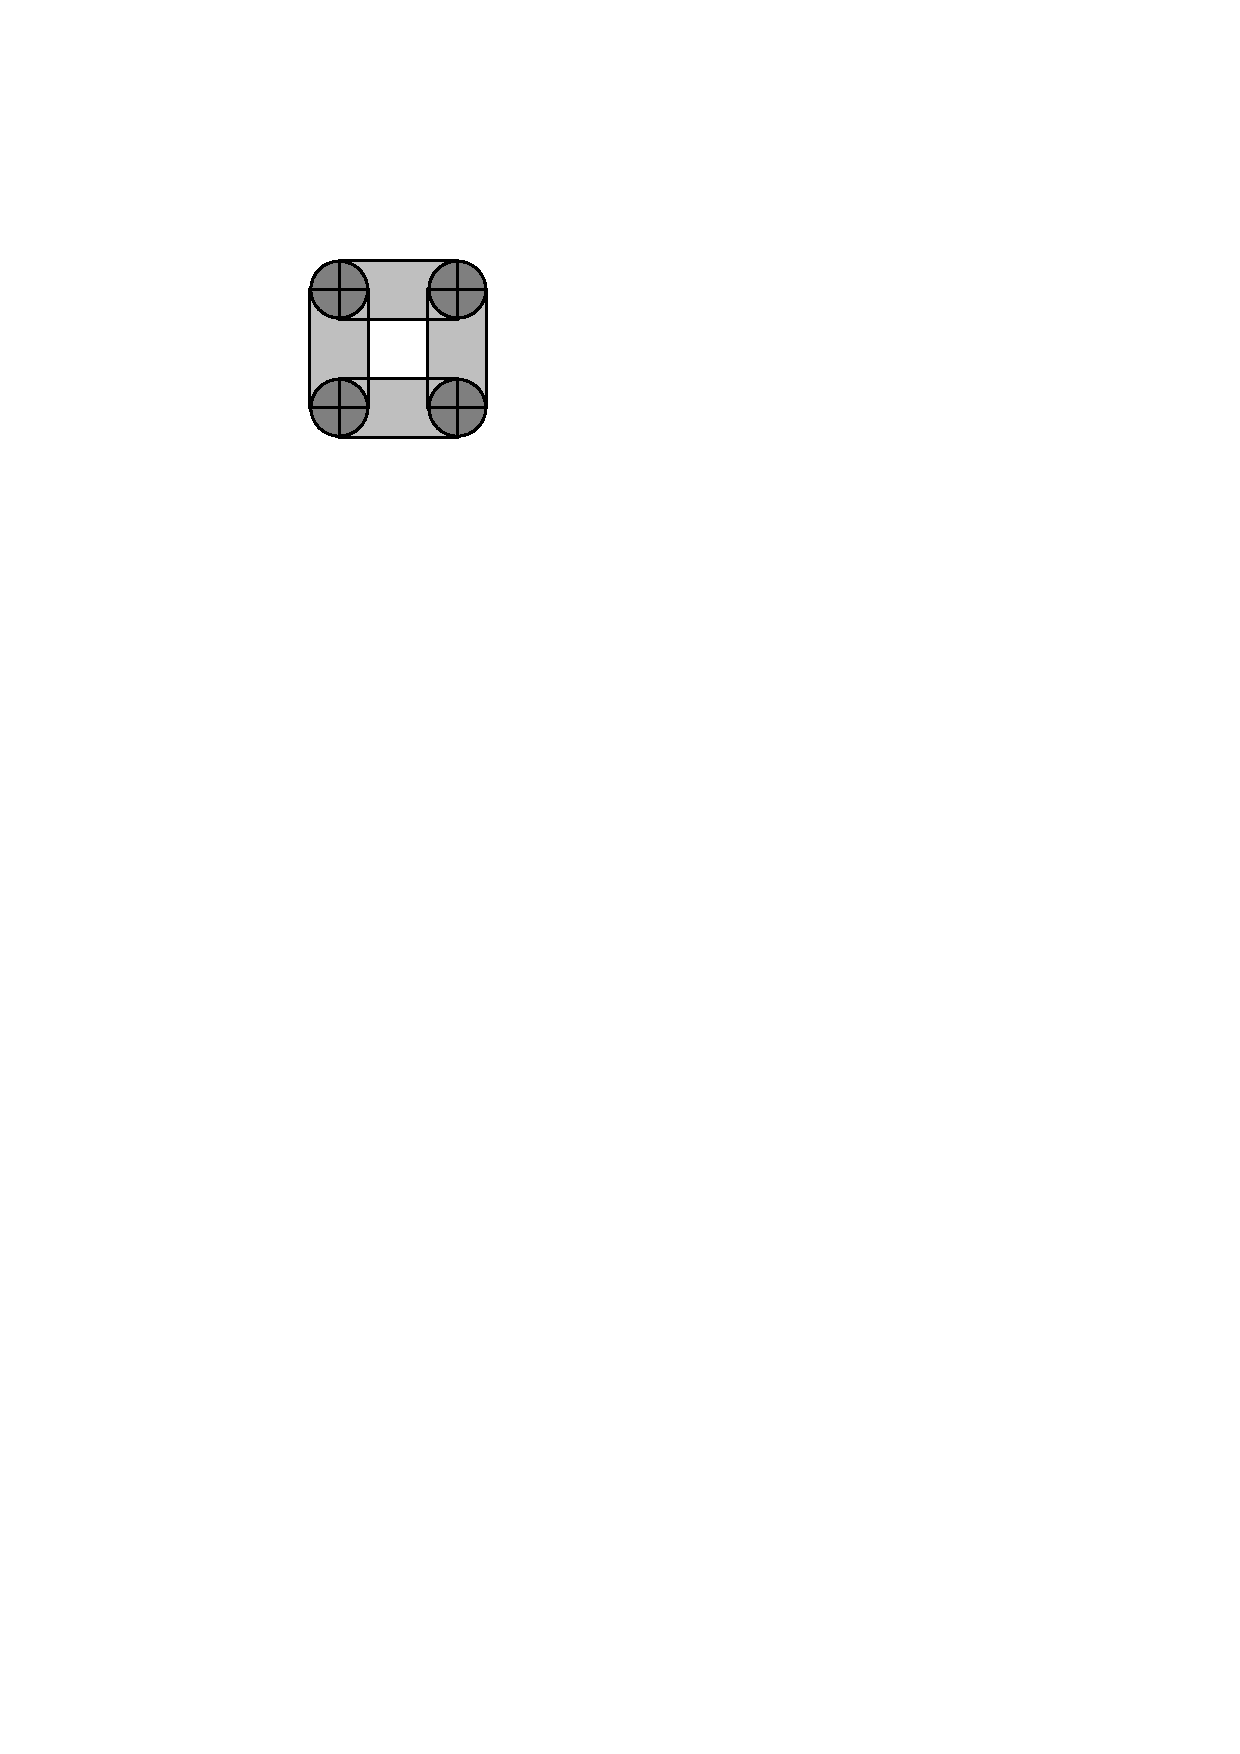
\includegraphics{Boolean_set_operations_2/fig/circles_rects}
    \end{center}
%    A general polygon with holes.
  \end{minipage}
  \vspace{2pt}
}

\ccIncludeExampleCode{Boolean_set_operations_2/circle_segment.cpp}

% ---------------------------------------------
\subsection{General Polygon Set Traits Adapter\label{bso_ssec:general_polygon_concept}}
% ---------------------------------------------

The concept \ccc{GeneralPolygon_2} and its generic model 
\ccc{General_polygon_2<ArrDirectionalXMonotoneTraits>} facilitate the 
production of general-polygon set traits classes. A model of the concept 
\ccc{GeneralPolygon_2} represents a simple point-set in the plane bounded 
by $x$-monotone curves. As opposed to the plain \ccc{Traits::Polygon_2} type 
defined by any traits class, it must define the type 
\ccc{X_monotone_curve_2}, which represents an $x$-monotone curve of the 
point-set boundary. It must provide a constructor from a range of such 
curves, and a pair of methods, namely \ccc{curves_begin()} and 
\ccc{curves_end()}, that can be used to iterate over the point-set boundary 
curves.
 
The class-template \ccc{General_polygon_2<ArrDirectionalXMonotoneTraits>}
models the concept \ccc{GeneralPolygon_2}. Its sole template parameter
must be instantiated with a model of the concept
\ccc{ArrangementDirectionalXMonotoneTraits_2} from which it obtains the 
\ccc{X_monotone_curve_2} type. It uses the geometric  operations
on this type provided by such a model to maintain a container of
directed curves of type \ccc{X_monotone_curve_2}, which represents a  
boundary of the general polygon.

The class-template
\ccc{Gps_traits_2<ArrDirectionalXMonotoneTraits,GeneralPolygon>}
models the concept \ccc{GeneralPolygonSetTraits_2}, and can be used to
instantiate the class template \ccc{General_polygon_set_2}.
It serves as an adapter for a geometric traits class, which models the
concept \ccc{ArrangementDirectionalXMonotoneTraits_2}.
It can be used for performing set-operations on general polygons.
The implementation of the adapter is rather simple, as it is derived
from the instantiated template-parameter \ccc{ArrXMonotoneTraits_2}
inheriting its necessary types and methods. It further exploits 
the methods provided by the instantiated parameter
\ccc{GeneralPolygon}, which is a model of the concept
\ccc{GeneralPolygon_2}. By default, the \ccc{GeneralPolygon} parameter
is defined as
\ccc{General_polygon_2<ArrangementDirectionalXMonotoneTraits_2>}.

The code excerpt listed below defines a general-polygon set type that
can be used to perform Boolean set-operations on point sets bounded by
the $x$-monotone curve type defined by the arrangement-traits class
\ccc{Arr_traits_2}, which is some representative model of the concept
\ccc{ArrangementDirectionalXMonotoneTraits_2}.
\begin{alltt}
#include <CGAL/General_polygon_2.h>
#include <CGAL/Gps_traits_2.h>

typedef CGAL::General_polygon_2<Arr_traits_2>               General_polygon_2;
typedef CGAL::Gps_traits_2<Arr_traits_2, General_polygon_2> Traits_2;
typedef CGAL::General_polygon_set_2<Traits_2>               General_polygon_set_2;
\end{alltt}

\lcTex{%
  \setlength{\BooleanSetOpsWidthRight}{3.4cm}
  \setlength{\BooleanSetOpsWidthLeft}{\BooleanSetOpsWidthLineReal}
  \addtolength{\BooleanSetOpsWidthLeft}{-\BooleanSetOpsWidthRight}
  \begin{minipage}{\BooleanSetOpsWidthLeft}
}
\label{fig:conics}
\begin{ccHtmlOnly}
  <p><center>
    <img src="./fig/tnr_m_g.gif" border=0 alt="Bezier curves" align=right>
  </center>
\end{ccHtmlOnly}
Instantiating the arrangement-traits \ccc{Arr_traits_2} above with the
traits class that handle B\'ezier curves \ccc{Arr_bezier_traits_2},
results with the definition of a general-polygon set type that can be
used to perform Boolean set-operations on point sets bounded by B\'ezier
curves.

The next example computes the intersection of two general polygons
bounded by B\'ezier curves read from two input files respectively. The
default input files our example uses (\ccc{char_g.dat} and
\ccc{char_m.dat}) define two general polygons shaped in the form of
the characters {\bf g} and {\bf m} in the Times New Roman font
respectively. Their intersection comprises nine simple polygons, as
depicted to the right.

% One is an ellipse given by $x^2 + 9y^2 - 9 = 0$,
% and the other is bounded by the two parabolic arcs whose underlying
% parabola are given by $x^2 + 2y - 4 = 0$, and $x^2 - 2y - 4 = 0$. The
% code in the example adapts the traits model that handles conics
% included with the \ccc{Arrangement_2} package.

\lcTex{%
  \end{minipage}\hspace{\BooleanSetOpsMinipageSpace}
  \begin{minipage}{\BooleanSetOpsWidthRight}
    \begin{center}
    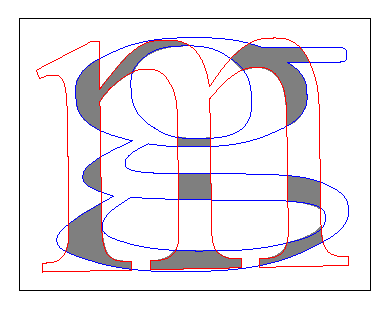
\includegraphics[width=4cm]{Boolean_set_operations_2/fig/tnr_m_g}
    \end{center}
  \end{minipage}
}

Recall that every B\'ezier curve is defined by a sequence of control
points that form chains (see Section~\ref{arr_ssec:tr_bez}. The last
control point of every curve must be identical to the first control
point of its successor. The function \ccc{read_Bezier_polygon()}
included in the example reads the curves from an input file until they
form a closed chain, which is assumed to be the outer boundary of the
polygon. If more curves are available, its starts constructing
polygons that correspond to holes in the area bounded by the outer
boundary. Note that this function is also responsible for subdividing
the input B\'ezier curves into $x$-monotone subcurves, as required by
the \ccc{Gps_traits_2} adapter.

\ccIncludeExampleCode{Boolean_set_operations_2/bezier_traits_adapter.cpp}

% ------------------------------------------
\subsection{Example - Aggregated Operations\label{bso_ssec:aggregated_gen_ops}}
% ------------------------------------------

In Section~\ref{bso_ssec:agg_ops} we describe how aggregated union
and intersection operations can be applied to a collection of ordinary
polygons or polygons with holes. Naturally, the aggregated operations
can be applied also to collections of general polygons. As was the
case with ordinary polygons, using aggregated operations is
recommended when the number of intersections of the input polygons
is of the same order of magnitude as the complexity of the result. If
this is not the case, computing the result incrementally may prove
faster.

\lcTex{%
  \setlength{\BooleanSetOpsWidthRight}{3.4cm}
  \setlength{\BooleanSetOpsWidthLeft}{\BooleanSetOpsWidthLineReal}
  \addtolength{\BooleanSetOpsWidthLeft}{-\BooleanSetOpsWidthRight}
  \begin{minipage}{\BooleanSetOpsWidthLeft}
}
\label{fig:disks}
\begin{ccHtmlOnly}
  <p><center>
    <img src="./fig/disks.gif" border=0 alt="Union of disks" align=right>
  </center>
\end{ccHtmlOnly}
The next example computes the union of eight unit discs whose centers are
placed a unit distance from the origin, as depicted to the right. The example
also allows users to provide a different number of discs through the command
line.
\lcTex{%
  \end{minipage}\hspace{\BooleanSetOpsMinipageSpace}
  \begin{minipage}{\BooleanSetOpsWidthRight}
    \begin{center}
    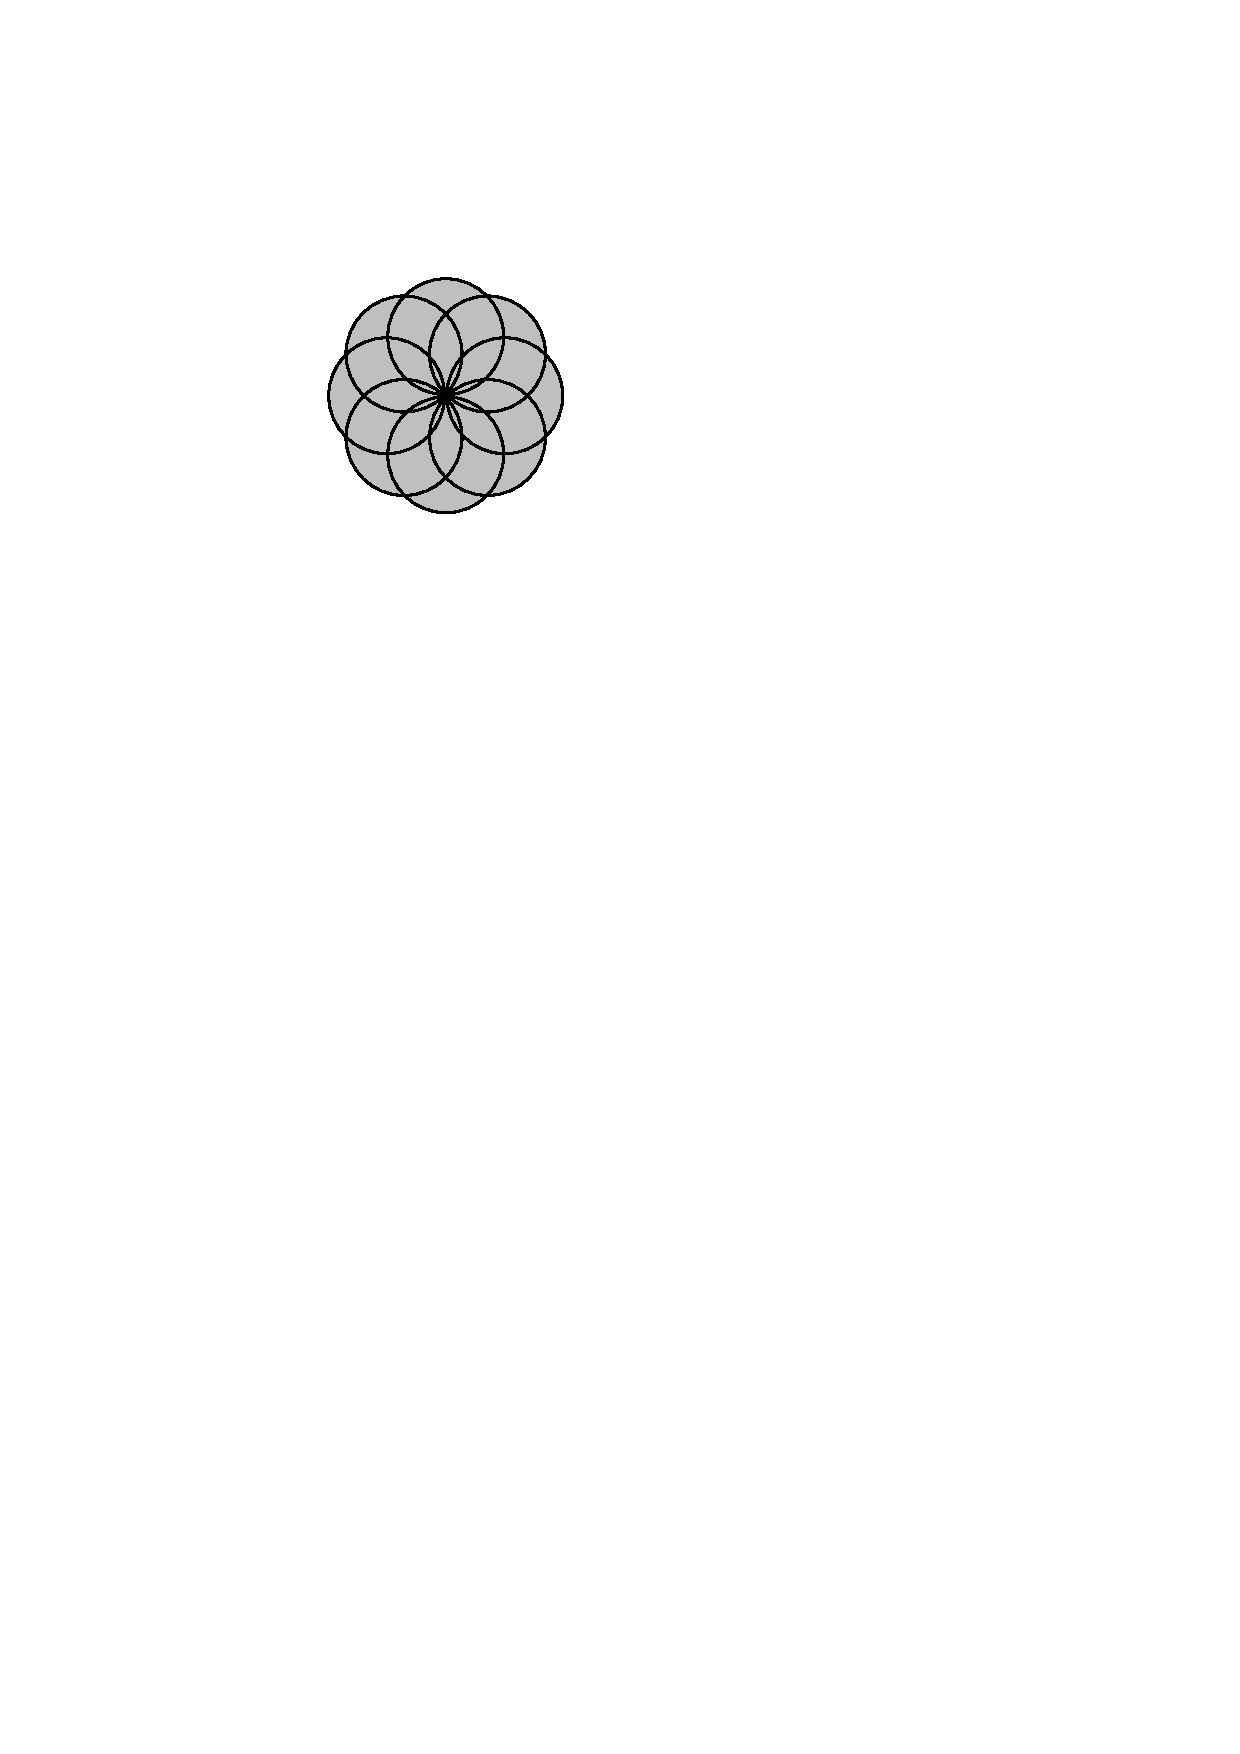
\includegraphics{Boolean_set_operations_2/fig/disks}
    \end{center}
%    Union of disks.
  \end{minipage}
\vspace{2pt}
}

\ccIncludeExampleCode{Boolean_set_operations_2/set_union.cpp}
